\documentclass{article}
\usepackage[utf8]{inputenc}
\usepackage{graphicx}
\graphicspath{ {./images/} }

\title{Exercise 9}
\author{garb }
\date{September 2021}

\begin{document}

\maketitle

\section{Diagram of the IsLeapYear function}
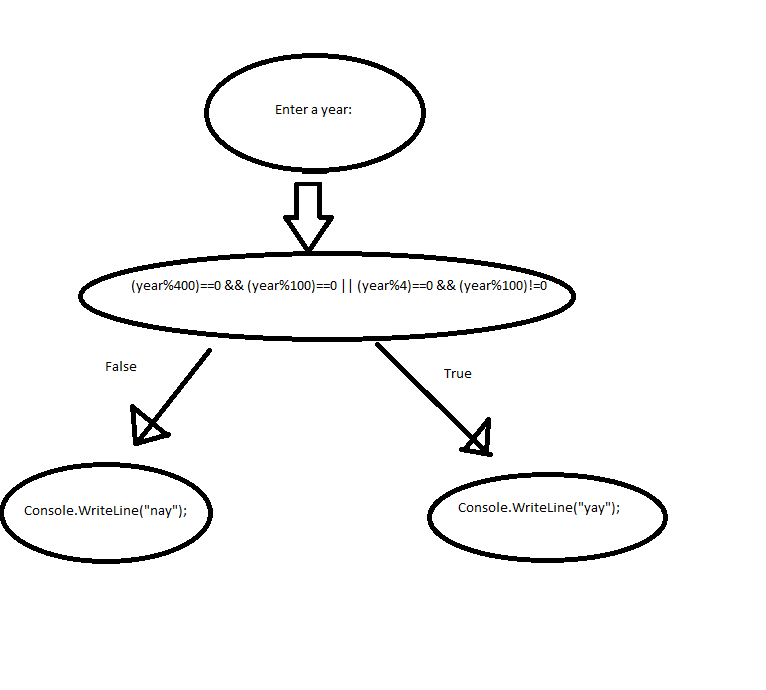
\includegraphics[width=120mm]{Exercise9.png}

After choosing an arbitrary year then the chosen year get put in the if statement (year%400)==0 && (year%100)==0 || (year%4)==0 && (year%100)!=0.
If year chosen year does not uphold the if-statement's criteria  then the method returns false which leads to the console printing "nay". If the year does uphold the if-statement's criteria then the console prints "yay.

\end{document}
